\noindent \textbf{Conjunto potencia.} \\
Considerando un \textit{cojunto de conjuntos} tal como $S$, donde $S$ es la clase de todos sus subconjuntos. Se le llama \textbf{conjunto potencia} de $S$ a esta clase de conjuntos y es denotado como $P(S)$. 
Donde su n\'umero de elementos en $P(S)$ es 2 elevado a la potencia de $n(S)$; eso es,

    \begin{center}
        $n(P(S)) = 2 P(S)^{n(S)}$.
    \end{center}

    \textbf{Ejemplo:}
        Suponga $S = \lbrace a,b,c\rbrace$ \\ \vspace{5px}

        Entonces $P(S) = \lbrace \emptyset, \lbrace a\rbrace,  \lbrace b\rbrace,  \lbrace c\rbrace,  \lbrace a, b\rbrace,  \lbrace a, c\rbrace, \lbrace b, c\rbrace, \lbrace a,b,c\rbrace \rbrace$.\\

    Se escribe $P(S) = \{X \,|\, X \subseteq A\}$. Nótese que todos los elementos de $P(S)$ son conjuntos.\\



% Ejemplos
\textbf{Ejemplos:} 
\begin{itemize}
    \item $P(\emptyset) = \{\emptyset\}$.
    \item Si $X = \{a\}$, entonces $P(X) = \{\emptyset, \{a\}\} = \{\emptyset, X\}$.
    \item Si $X = \{\emptyset, \{\emptyset\}, \{a\}, \{b\}, \{\emptyset, a\}, \{\emptyset, b\}, \{a, b\}, X\}$.
\end{itemize}


Como para cada subconjunto $X$, $\emptyset \subseteq X$, entonces $P(X) = \emptyset$ tendrá por lo menos dos elementos que son $\emptyset$ y $X$.

% Teorema 1
\textbf{Teorema 1.} \\
Para cualesquiera conjuntos $A$ y $B$, $$P(A \cup B) \supseteq P(A) \cup P(B).$$

\textbf{Demostración.}Tenemos que 
\begin{align*}
X \in P(A) \cup P(B) &\Rightarrow X \subseteq A \lor X \subseteq B \\
&\Rightarrow X \subseteq A \cup B \\
&\Rightarrow X \in P(A \cup B).
\end{align*}


% Ejemplo que muestra que la otra inclusión no siempre se cumple
\textbf{Ejemplo.} La otra inclusión no siempre se cumple, veamos un ejemplo. Consideremos los conjuntos $A = \{1, 2, 3\}$ y $B = \{2, 3, 4\}$. Tenemos entonces:
\begin{align*}
    P(A) &= \{\emptyset, \{1\}, \{2\}, \{3\}, \{1, 2\}, \{1, 3\}, \{2, 3\}, \{1, 2, 3\}\} \\
    P(B) &= \{\emptyset, \{2\}, \{3\}, \{4\}, \{2, 3\}, \{3, 4\}, \{2, 4\}, \{2, 3, 4\}\}
\end{align*}
Y la unión de los conjuntos potencia es:
\begin{align*}
    P(A) \cup P(B) &= \{\emptyset, \{1\}, \{2\}, \{3\}, \{4\}, \{1, 2\}, \{1, 3\}, \{2, 3\}, \{3, 4\}, \{1, 2, 3\}, \{2, 3, 4\}\}
\end{align*}
Por otro lado, $A \cup B = \{1, 2, 3, 4\}$, de manera que:

%% NO SE CÓMO ACOMODAR ESTO :C
\begin{align}
    P(A \cup B) &= \{\emptyset, \{1\}, \{2\}, \{3\}, \{4\}, \{1, 2\}, \{1, 3\}, \{1, 4\}, \{2, 3\}, \{2, 4\}, \{3, 4\}, \{1, 2, 3\}, \{1, 2, 4\}, \{1, 3, 4\}, \{2, 3, 4\}, \{1, 2, 3, 4\}\}\\
\end{align}
%%%%%%%%%%%%%%%%%%%%%%%%%%%%%%%%%%%%%%%%%%%%%%%%%%%%%%%%%%%%%%%

Observamos que $ \{1, 2, 3, 4\} \subset P(A \cup B)$, y $\{1, 2, 3, 4\} \not\subset P(A) \cup P(B)$. Por lo tanto, la otra inclusión no siempre se cumple.\\

% Teorema 2
\textbf{Teorema 2.}\\ Para cualesquiera conjuntos $A$ y $B$, $$P(A \cap B) = P(A) \cap P(B).$$

\textbf{Demostración.} Tenemos que 
\begin{align*}
X \in P(A) \cap P(B) &\Leftrightarrow X \in P(A) \land X \in P(B) \\
&\Leftrightarrow X \subseteq A \land X \subseteq B \\
&\Leftrightarrow X \subseteq A \cap B \\
&\Leftrightarrow X \in P(A \cap B).
\end{align*}


\vspace{10px} \noindent  \textbf{Conjunto producto.} \\    
 Sean $A$ y $B$ dos conjuntos. El \textit{conjunto producto} de $A$ y $B$, expresado como $A \times B$, est\'a formado por todas las parejas ordenadas $(a,b)$ donde $a \in A$ y $b \in B$:

        \begin{center}
            $A \times B = \lbrace (a,b) : a \in A, b \in B\rbrace$.
        \end{center}

   \textbf{Ejemplo:}  Sea $A = \lbrace a, b \rbrace$, $B = \lbrace 1, 2 \rbrace$ \\

    El conjunto producto de $A \times B = \lbrace(a, 1), (a, 2), (b, 1), (b, 2)\rbrace$. \\
        

    Nota. El producto de un conjunto por sí mismo, $A \times A$, se denota por $A^2$. \vspace{5px}\\
\noindent \textbf{Conjunto producto de $A \times B  \times C.$} \\
         
   \noindent\textbf{Ejemplo:} Sea $A = \lbrace 1, 2 \rbrace$,
    $B = \lbrace x, y, z \rbrace$ y 
    $C = \lbrace 3, 4 \rbrace$.  Encontrar $A \times B  \times C.$ \\

    \noindent$A \times B  \times C$ consta de todos los elementos ordenados de $(a,b,c)$ donde $a \in A$, $b \in B$, $c \in C$. Estos elementos de $A \times B  \times C.$ se pueden obtener sistem\'aticamente mediante el llamado diagrama de \'arbol. \\

    Donde $n(A) = 2$, $n(B) = 3$ y $n(C) = 2$,  por lo que:

    \begin{center}
       $n(A \times B  \times C) = 12 = n(A) \cdot n(B) \cdot n(C)$
    \end{center}

     \vspace{10px}
     
\begin{multicols}{3}

    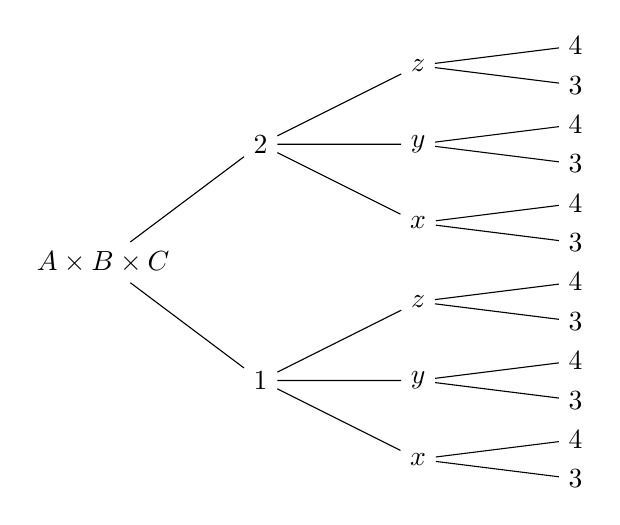
\begin{tikzpicture}[level distance=2cm,
      level 1/.style={sibling distance=3cm},
      level 2/.style={sibling distance=1cm},
      level 3/.style={sibling distance=0.5cm},grow=right]
  
      \node {$A \times B \times C$}
        child { node {$1$}
              child { node {$x$}
                child {
                  node {$3$}
                }
                child {
                  node {$4$}
                }
              }
              child { node {$y$}
                child {
                  node {$3$}
                }
                child {
                  node {$4$}
                }
              }
              child {   node {$z$}
                child {
                  node {$3$}
                }
                child {
                  node {$4$}
                }
              }
        }
        child {  node {$2$}
          child {    node {$x$}
            child {
              node {$3$}
            }
            child {
              node {$4$}
            }
          }
          child {  node {$y$}
            child {
              node {$3$}
            }
            child {
              node {$4$}
            }
          }
          child {    node {$z$}
            child {
              node {$3$}
            }
            child {
              node {$4$}
            }
          }
        };
    
    \end{tikzpicture}
        
    \columnbreak
    \hspace{1cm}
    \columnbreak
    
    \begin{itemize}
     \renewcommand\labelitemi{}
        \item $(2,z,4)$
        \item $(2,z,3)$
        \item $(2,y,4)$
        \item $(2,y,3)$
        \item $(2,x,4)$
        \item $(2,x,3)$
                 
        \item $(1,z,4)$
        \item $(1,z,3)$
        \item $(1,y,4)$
        \item $(1,y,3)$
        \item $(1,x,4)$
        \item $(1,x,3)$
     \end{itemize}
        
\end{multicols}
        


\\ 

\vspace{10px}\noindent \textbf{Conjuntos Autocontenidos.} \\ Un conjunto se considera \textit{autocontenido} cuando todos sus elementos también son elementos de otro conjunto más grande, es decir, cuando está completamente contenido dentro de otro conjunto.

\noindent \textbf{Definición.}

\noindent Formalmente, un conjunto $A$ se llama autocontenido si para todo elemento $x$ en $A$, $x$ también es un elemento de otro conjunto $B$.

\[
A \subseteq B \quad \text{o} \quad B \supseteq A
\]

\noindent Esto significa que $A$ es un subconjunto de $B$, o equivalentemente, $B$ es un superconjunto de $A$.

\noindent \textbf{Ejemplos:}

\begin{enumerate}
  \item Si consideramos los conjuntos $A = \{1, 2\}$ y $B = \{1, 2, 3, 4\}$, entonces $A$ es un subconjunto de $B$, es decir, $A \subseteq B$, porque todos los elementos de $A$ (1 y 2) también están en $B$.
  
  \item Tomemos los conjuntos $C = \{a, b, c\}$ y $D = \{a, b, c, d, e\}$. En este caso, $C$ es un subconjunto de $D$ ya que todos los elementos de $C$ (a, b y c) también están en $D$.
  
  \item Si consideramos el conjunto vacío $\emptyset$, este conjunto es un subconjunto de cualquier otro conjunto. Por ejemplo, $\emptyset \subseteq A$ para cualquier conjunto $A$, ya que no contiene ningún elemento que no esté en $A$.
\end{enumerate}